\documentclass[12pt,a4paper]{article}

% --- Encoding and math ---
\usepackage[utf8]{inputenc}
\usepackage[T1]{fontenc}
\usepackage{amsmath,amssymb,amsthm}

% --- Graphics and layout ---
\usepackage{graphicx}
\usepackage{geometry}
\geometry{margin=1in}
\usepackage{microtype}
\microtypesetup{expansion=false}

% --- TikZ for figures ---
\usepackage{tikz}
\usetikzlibrary{arrows.meta, positioning, shapes, shadows, calc, decorations.pathmorphing}
\usepackage{pgfplots}
\pgfplotsset{compat=1.18}
\def\wave{decorate, decoration={coil, aspect=0}}

% --- Tables ---
\usepackage{booktabs}
\usepackage{caption}
\captionsetup{justification=centering}

% --- Listings ---
\usepackage{listings}
\usepackage{xcolor}

\lstset{
  basicstyle=\ttfamily\small,
  breaklines=true,
  breakatwhitespace=true,
  columns=fullflexible,
  keepspaces=true,
  postbreak=\mbox{\textcolor{gray}{$\hookrightarrow$}\space}
}

% --- Section formatting ---
\usepackage{titlesec}

% --- Floats, spacing, paragraph style ---
\usepackage{float}
\usepackage{setspace}
\usepackage{parskip}
\usepackage{placeins}

% --- Verbatim with wrapping ---
\usepackage{fancyvrb}
\usepackage{fvextra}
\usepackage{listings}

% --- Numeric tables ---
\usepackage{siunitx}
\sisetup{
    table-number-alignment = center,
    table-text-alignment   = center
}

% --- Input path flexibility ---
\makeatletter
\def\input@path{{./}{./tables/}}
\makeatother

% --- Line spacing ---
\onehalfspacing
\sloppy

% --- Citations and links ---
\usepackage[authoryear]{natbib}
\usepackage{hyperref}
\hypersetup{
  colorlinks=true,
  linkcolor=black,
  citecolor=black,
  urlcolor=black
}
\usepackage{cleveref}

% Format abstract full page
\makeatletter
\renewenvironment{abstract}{
    \begin{center}
        {\large\bfseries \abstractname\vspace{-.5em}\vspace{0pt}}
    \end{center}
}{}
\makeatother

\title{Embodied Regulatory Intelligence \\
\Large in Chaotic Physical Systems: \\
\small A Neurosymbolic Cognitive Architecture Coupled to Navier--Stokes Dynamics}

\author{
John H. Cragin\\
Independent Researcher\\
\texttt{john.cragin@outlook.com}\\
ORCID: \url{https://orcid.org/0009-0001-5204-5732}
}


\date{\today{}}

\begin{document}

\maketitle

\thispagestyle{empty}

\begin{abstract}
Safely embodying synthetic cognition in physical systems demands agents capable of self-regulation to prevent unintended harm or instability. This paper introduces a bidirectional coupling between a neurosymbolic Regulatory Intelligence (RI) architecture and a custom 2D incompressible Navier--Stokes solver. The RI agent, implemented as SpiralBrain v3.0 \cite{SpiralBrainV3}, is a Python-based neurosymbolic system that runs locally on standard hardware (e.g., a laptop).

The agent’s perceptual module (the Sensus lobe) ingests aggregate flow statistics (a fixed 128-dimensional vector of velocity and pressure summaries) and contextually modulates viscosity ($\nu$) and timestep ($\Delta t$) in response to turbulence, treated as a metacognitive stressor that elevates Hazard~$H$. This triggers low-gain, context-sensitive homeostatic throttling to preserve internal coherence without directive control.

A sequential observer-effect protocol evaluates carryover effects and regulatory restraint across baseline, passive observation, naive regulation, and adaptive RI conditions. Results indicate bounded flows with emergent multi-vortex structures (peak speed $\approx 0.236$, average vorticity $\approx 0.040$), perfect elastic absorption (post-decoupling $\phi_{\max}=0^\circ$), epistemic parity under adaptive regulation ($\phi_{\max}$ comparable to observer conditions; regulatory sensitivity $=0^\circ$), and 100\% numerical stability across runs. No divergences or regime shifts were observed. Due to the small sample size ($n=4$) and bounded experimental scope, these findings characterize behavior within the tested coupling envelope and warrant replication under broader conditions.

Unlike control-theoretic or Physics-Informed Neural Network (PINN) approaches that prioritize solution accuracy or impose trajectory constraints, this work adopts a viability-first paradigm: turbulence serves as a stressor to evaluate intelligent restraint rather than solution fidelity. Within the tested regime, these findings provide empirical evidence for the potential of RI architectures in safe, homeostatic embodiment within chaotic physical loops, with possible extensions to simplified embodied control contexts such as robotics or multi-physics agents.
\end{abstract}

\section*{Nomenclature}

\begin{description}
\item[CCS] Cognitive Coherence Score
\item[CFD] Computational Fluid Dynamics
\item[EPCI] Epistemic Parity Coherence Index
\item[NS] Navier--Stokes
\item[PINNs] Physics-Informed Neural Networks
\item[RI] Regulatory Intelligence
\item[SEC] Stability, Equilibrium, Coherence
\end{description}

\section{Introduction}

Regulatory Intelligence (RI) is a paradigm of synthetic cognition that prioritizes internal viability and coherence over external task optimization. Rather than maximizing performance objectives, an RI system maintains bounded internal stability through homeostatic feedback mechanisms. In the present architecture, perceptual inputs are processed through a dedicated sensory interface (the Sensus module) into a structured internal state representation encoding stability, equilibrium, and coherence. Stress proxies (denoted Hazard~$H$) track deviations from viable operating regimes, and adaptive throttling mechanisms act to restore coherence only when necessary. This design emphasizes restraint: regulation is applied contextually and minimally, avoiding dominance over the coupled environment.

The neurosymbolic implementation of this architecture, SpiralBrain v3.0, integrates symbolic rules for contextual decision-making with neural-style homeostatic mechanisms for elastic stress response. This combination enables structured yet adaptive modulation while preserving interpretability at the regulatory level, without requiring disclosure of full internal implementation details.

However, prior work in embodied cognition often prioritizes task performance or prediction accuracy, which can risk instability when agents are coupled to inherently chaotic physical systems. We address this critical gap by coupling a neurosymbolic RI agent (SpiralBrain v3.0) to 2D Navier--Stokes turbulence as a metacognitive stressor. The agent processes flow statistics to modulate physical parameters, demonstrating how homeostatic regulation enables safe embodiment without divergence or over-intervention in low-Reynolds-number regimes. Results indicate perfect elastic absorption, epistemic parity, and 100\% stability across limited runs (n=4), providing preliminary support for RI's potential in chaotic physical loops. The present study is intended as a proof-of-concept demonstration of viability-first embodiment rather than a claim of task-optimal or production-ready control. The modulation strategy (low-gain, infrequent adjustments) may bias toward success in this setup; future work should test higher Re or 3D flows for robustness.

The 2D Navier--Stokes equations provide a canonical nonlinear, self-advecting chaotic system that serves as an ideal testbed for evaluating Hazard H elevation and homeostatic response without requiring high-resolution CFD accuracy. Unlike simpler chaotic systems (e.g., Lorenz equations or low-dimensional ODEs), Navier--Stokes provides spatially extended, multi-scale, physically grounded chaos that mirrors real-world embodiment challenges.

\textbf{Core contribution.} We present a unified synthetic cognitive architecture (SpiralBrain v3.0) that can (i) remain elastically stable under sustained interaction with a chaotic physical simulator (2D Navier--Stokes), (ii) modulate physical parameters contextually without exerting directive control, and (iii) exhibit epistemic regulation characterized by intelligent restraint, quantified through observer-effect metrics.

The central question is whether an RI agent can remain coupled to a chaotic system while exercising intelligent restraint, i.e., modulating physical parameters only when needed to protect its internal coherence, without attempting to dominate the dynamics.

\section{Background and Related Work}

Physics-Informed Neural Networks (PINNs) \cite{Raissi2019} integrate governing equations such as Navier--Stokes into a loss function to improve solution accuracy or enable inverse problem solving. In contrast, the present work does not treat the physical system as a target to be solved or controlled, but rather as a metacognitive stressor for evaluating regulatory behavior. Turbulence functions as a metacognitive stressor that elevates Hazard (H), allowing regulatory behavior—particularly restraint and homeostatic throttling—to be evaluated independently of solution accuracy. The distinction is therefore not one of model fidelity, but of objective: optimization versus viability.

This work builds on foundational ideas in embodied cognition, such as Rodney Brooks' subsumption architecture \cite{Brooks1991}, which emphasizes layered, reactive behaviors over centralized planning, and Andy Clark's extended mind hypothesis \cite{Clark1998}, where cognitive processes extend into the environment. Our approach integrates these by treating the physical simulator as an extended cognitive resource that the agent modulates homeostatically rather than controls hierarchically.

This viability-first stance follows the Regulatory Intelligence paradigm of geometric homeostasis and elastic cognition \cite{Cragin2026RI}.

Symbolic–Emotional Calibration follows the SEC framework defined in \cite{Cragin2026SEC}.

While drawing on CFD numerics and control-style coupling, this work is framed as a cognitive systems study using fluid dynamics as a testbed for regulatory intelligence.

\begin{table}[htbp]
\centering
\caption{Contrasting Physics-Informed Neural Networks (PINNs) with Regulatory Intelligence (RI).}
\label{tab:contrast}
\begin{tabular}{@{} p{4.5cm} p{5cm} p{5.5cm} @{}}
\toprule
\textbf{Dimension} & \textbf{PINNs} & \textbf{Regulatory Intelligence} \\
\midrule
Objective          & Solution accuracy and inversion problems & Prioritizes internal viability and coherence over task performance \\
Physics Role       & Governing equations as hard/soft constraints in loss function & Physical system as metacognitive stressor elevating Hazard H \\
Metric             & Residual / solution error norms & $\phi_{\max}$ (perturbation angle), EPCI (epistemic parity) \\
\bottomrule
\end{tabular}
\end{table}

\section{System Architecture}

SpiralBrain v3.0 is a neurosymbolic cognitive architecture that integrates neural processing with symbolic reasoning for adaptive regulation. Symbolic rules govern parameter modulation based on flow state vectors, integrated with neural homeostasis via SEC bands to ensure viability-preserving actions. This hybrid approach enables context-aware restraint, treating turbulence as a stressor rather than a control target, without exposing proprietary internals.

\subsection{Implementation Environment}

The SpiralBrain v3.0 architecture is implemented in Python and executes in a local computational environment, such as a laptop running Visual Studio Code. This lightweight design enables real-time bidirectional coupling with the Navier–Stokes solver without requiring high-performance computing resources.

\begin{figure}[H]
\centering
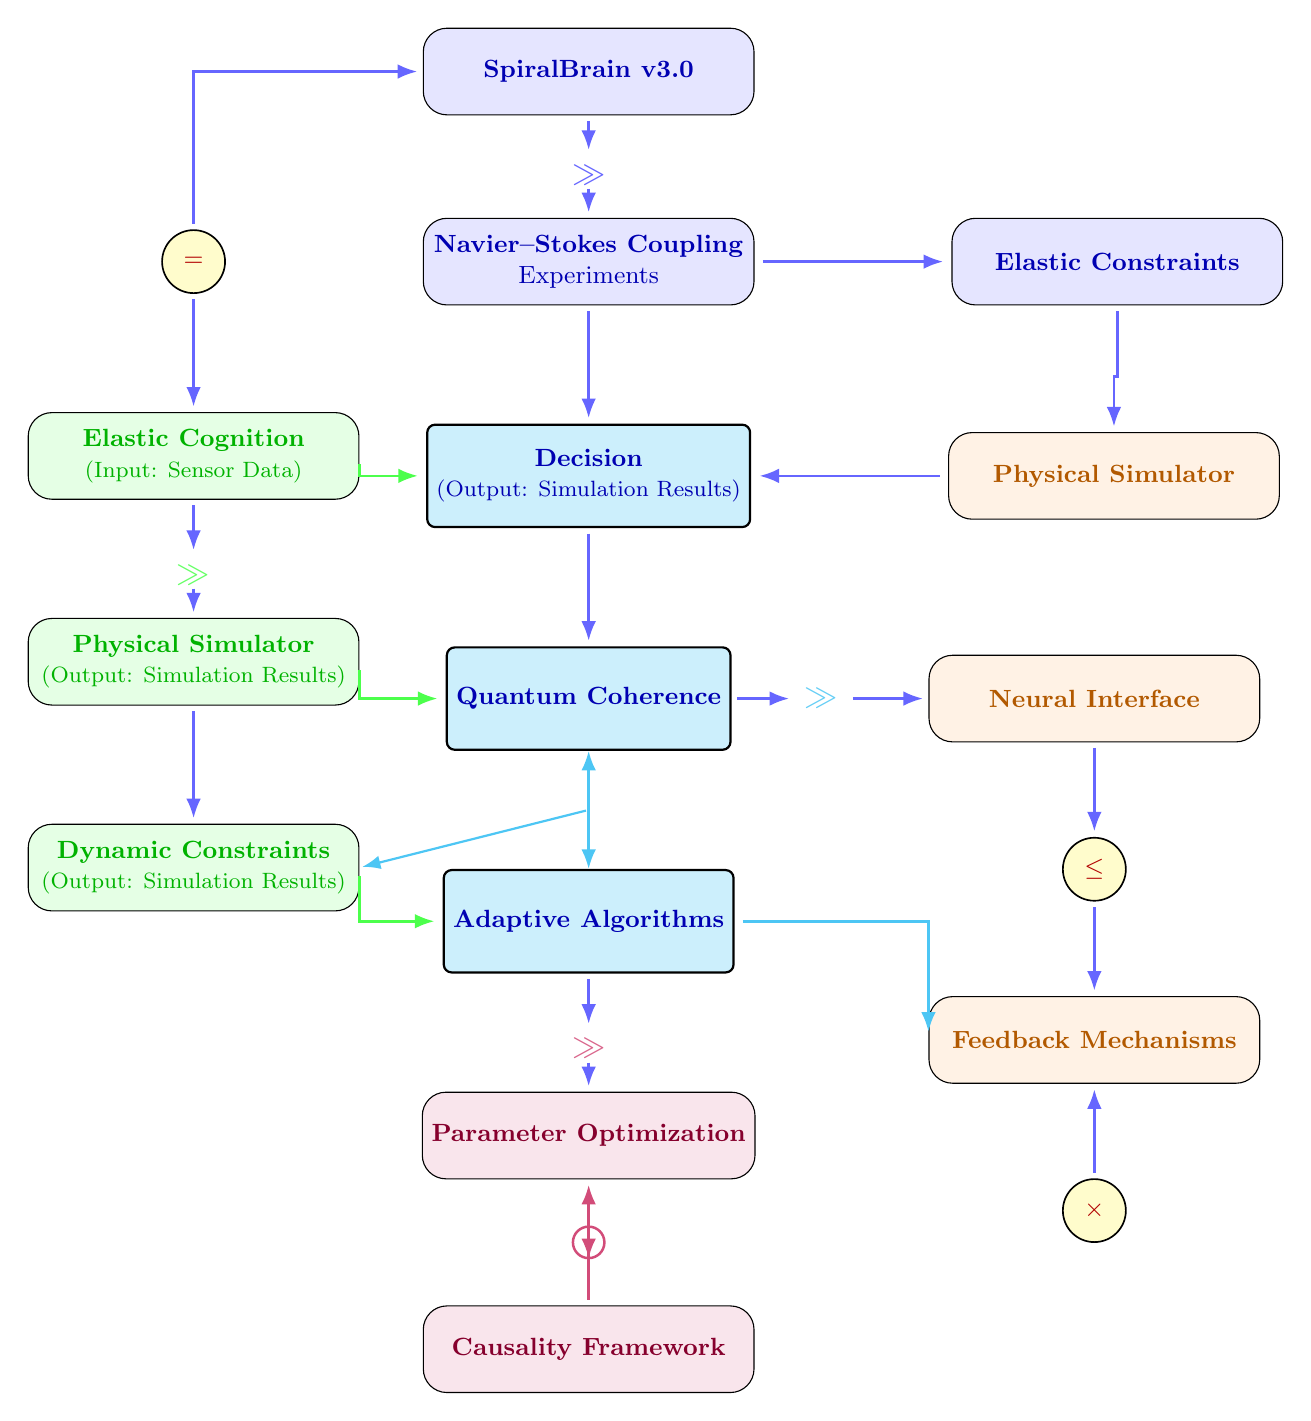
\begin{tikzpicture}[
    font=\small,
    >=Latex,
    node distance=15mm and 25mm,
    box/.style={draw, rounded corners=3mm, minimum width=42mm, minimum height=11mm, align=center, fill=white},
    decision/.style={draw, rounded corners=1mm, minimum width=32mm, minimum height=13mm, align=center, fill=cyan!20, text=blue!70!black, line width=0.8pt},
    mainbox/.style={box, fill=blue!10, text=blue!70!black},
    leftbox/.style={box, fill=green!10, text=green!70!black},
    rightbox/.style={box, fill=orange!10, text=orange!70!black},
    bottombox/.style={box, fill=purple!10, text=purple!70!black},
    circ/.style={draw, circle, minimum size=8mm, inner sep=0pt, fill=yellow!20, text=red!70!black, line width=0.6pt},
    line/.style={-Latex, line width=0.9pt, blue!60},
    vline/.style={line, shorten >=2pt, shorten <=2pt},
    hline/.style={line, shorten >=3pt, shorten <=3pt},
    bidirect/.style={<->, line width=0.9pt, cyan!70},  % Two-way arrow style
    centerleft/.style={<-, line width=0.8pt, cyan!70, shorten >=1pt, shorten <=1pt}  % Center left arrow
]

% ===== TOP SECTION =====
\node[mainbox] (sb) {\textbf{SpiralBrain v3.0}};

% Coupling experiments below SB
\node[mainbox, below=13mm of sb] (ns) {\textbf{Navier--Stokes Coupling}\\Experiments};

% Elastic constraints to the right
\node[mainbox, right=of ns] (elastic) {\textbf{Elastic Constraints}};

% ===== LEFT COLUMN =====
% Equal circle left of NS
\node[circ, left=of ns] (eqL) {$=$};

% Elastic cognition below left circle
\node[leftbox, below=of eqL] (ec) {\textbf{Elastic Cognition}\\\footnotesize(Input: Sensor Data)};

% Left physical simulator
\node[leftbox, below=of ec] (psL) {\textbf{Physical Simulator}\\\footnotesize(Output: Simulation Results)};

% Dynamic constraints
\node[leftbox, below=of psL] (dc) {\textbf{Dynamic Constraints}\\\footnotesize(Output: Simulation Results)};

% ===== CENTER COLUMN (Decision boxes) =====
% Decision box below NS
\node[decision, below=of ns] (dec) {\textbf{Decision}\\\footnotesize(Output: Simulation Results)};

% Quantum coherence below decision
\node[decision, below=of dec] (qc) {\textbf{Quantum Coherence}};

% Adaptive algorithms below quantum coherence
\node[decision, below=of qc] (aa) {\textbf{Adaptive Algorithms}};

% Parameter optimization below adaptive algorithms
\node[bottombox, below=of aa] (po) {\textbf{Parameter Optimization}};

% Causality framework at bottom
\node[bottombox, below=16mm of po] (cf) {\textbf{Causality Framework}};

% ===== RIGHT COLUMN =====
% Right physical simulator
\node[rightbox, right=of dec] (psR) {\textbf{Physical Simulator}};

% Neural interface
\node[rightbox, right=of qc] (ni) {\textbf{Neural Interface}};

% Less-than-or-equal circle
\node[circ, below=12mm of ni] (leqR) {$\leq$};

% Feedback mechanisms
\node[rightbox, below=12mm of leqR] (fb) {\textbf{Feedback Mechanisms}};

% Multiply circle
\node[circ, below=12mm of fb] (mul) {$\times$};

% ===== DECORATIVE ELEMENTS =====
% Flow indicators
\node[font=\bfseries\large, above=3mm of ns, text=blue!60] (gt1) {$\gg$};
\node[font=\bfseries\large, above=3mm of psL, text=green!60] (gt2) {$\gg$};
\node[font=\bfseries\large, right=8mm of qc, text=cyan!60] (gt3) {$\gg$};
\node[font=\bfseries\large, above=3mm of po, text=purple!60] (gt4) {$\gg$};

% ===== CONNECTIONS =====

% Top vertical flow
\draw[vline] (sb) -- (gt1);
\draw[vline] (gt1) -- (ns);

% Horizontal from NS to Elastic Constraints
\draw[hline] (ns.east) -- (elastic.west);

% Elastic Constraints down to right Physical Simulator
\draw[vline] (elastic.south) |- ++(0,-9mm) -| (psR.north);

% Left equal circle connections
\draw[vline] (eqL) |- (sb.west);
\draw[vline] (eqL) -- (ec);

% Left column vertical
\draw[vline] (ec) -- (gt2);
\draw[vline] (gt2) -- (psL);

\draw[vline] (psL) -- (dc);

% Center column vertical (except between qc and aa)
\draw[vline] (ns) -- (dec);
\draw[vline] (dec) -- (qc);

% Quantum Coherence to Adaptive Algorithms is now bidirectional
\draw[bidirect] (qc) -- (aa);
\draw[vline] (aa) -- (gt4);
\draw[vline] (gt4) -- (po);

% Center arrow from midpoint of qc-aa connection to Dynamic Constraints
\draw[centerleft] (dc.east) -- ($(qc)!0.5!(aa)$);

% Decision to right physical simulator
\draw[hline] (psR.west) -- (dec.east);

% Quantum coherence to neural interface
\draw[vline] (qc.east) -- (gt3);
\draw[vline] (gt3) -- (ni.west);
%\draw[hline] (qc.east) -- (ni.west);

% Neural interface to feedback chain
\draw[vline] (ni.south) -- (leqR);
\draw[vline] (leqR) -- (fb);
\draw[vline] (mul) -- (fb);

% Cross connections from left to center
\draw[hline, green!70] (ec.east) |- (dec.west);
\draw[hline, green!70] (psL.east) |- (qc.west);
\draw[hline, green!70] (dc.east) |- (aa.west);
% Note: Connection from dc to aa is replaced by centerleft arrow from midpoint

% Adaptive algorithms to feedback
\draw[hline, cyan!70] (aa.east) -| (fb.west);

% Parameter optimization to causality with loop
\draw[vline, purple!70] (cf.north) -- (po);
% Add small loop indicator
\draw[line, purple!70] ($(po.south)!0.5!(cf.north)$) circle (2mm);
\draw[line, purple!70] ($(po.south)!0.5!(cf.north)$) ++(0,2mm) -- ++(0,-4mm);

\end{tikzpicture}
\caption{\raggedright System architecture showing bidirectional coupling between SpiralBrain v3.0 and the Navier--Stokes simulator, including perceptual ingestion, regulatory decision pathways, and constrained feedback mechanisms.}
\label{fig:system_architecture}
\end{figure}

The Navier--Stokes equations describe the motion of viscous fluid substances, here solved in 2D incompressible form using a finite-difference method on a 64×64 uniform grid. Initial conditions consist of a Gaussian perturbation centered at (0.5, 0.5) to seed turbulence, with no-slip boundary conditions enforcing zero velocity at domain edges. Pressure is projected using Successive Over-Relaxation (SOR) to ensure incompressibility. Coupling occurs bidirectionally: every 10 simulation steps, the brain receives summarized flow statistics and modulates viscosity ($\nu$) and timestep ($\Delta t$) to influence flow evolution contextually. This custom solver prioritizes chaotic dynamics over numerical precision, providing a realistic yet computationally tractable testbed for regulatory intelligence without the overhead of production CFD codes.

Cognitive influence is restricted to: \\ 
(i) low-gain $\nu$ modulation, \\ 
(ii) low-gain $\Delta t$ modulation, \\ 
(iii) updates every 10 steps; no changes to velocity/pressure fields, boundaries, or forcing.

This design ensures the agent modulates physical parameters contextually without exerting directive control.

High-level overview of SpiralBrain's decision/action pathway: Sensory inputs from the Sensus lobe are processed into SEC vectors, which are evaluated against Hazard $H$ thresholds. If stress exceeds elastic limits, homeostatic bands trigger adaptive throttling, modulating parameters like viscosity and timestep to restore coherence without direct control.

Grid: 64×64; Initial condition: Gaussian perturbation centered at (0.5, 0.5); Adaptation frequency: every 10 steps; Input summarization: mean/std/max/min of (u, v, p) $\rightarrow$ padded to 128D vector.

\section{Experimental Design}

\subsection{Physical System}

The physical environment consists of a two-dimensional incompressible Navier--Stokes system solved on a 64×64 grid using a finite-difference formulation with pressure projection via successive over-relaxation. No-slip boundary conditions are applied on all domain boundaries. The initial condition is a centered Gaussian velocity perturbation at (0.5, 0.5), producing a decaying vortex structure characteristic of low-to-moderate Reynolds number flow. Navier--Stokes dynamics were chosen not for physical fidelity but because they provide a well-studied, self-advecting chaotic system with intrinsic instability that reliably elevates regulatory stress without external forcing.

All simulations are executed for a fixed horizon of 50 timesteps. No external forcing or boundary modulation is applied at any point during execution.

\subsection{Cognitive Coupling}

The cognitive system observes the physical state through aggregate flow statistics, including mean and maximum speed and vorticity summaries, projected into a fixed 128-dimensional observation vector. This projection is invariant across conditions.

Cognitive influence on the physical system is strictly limited to low-gain modulation of kinematic viscosity ($\nu$) and simulation timestep ($\Delta t$), applied at fixed intervals of ten timesteps. Direct manipulation of velocity fields, pressure fields, boundary conditions, or external energy injection is explicitly prohibited.

This design ensures that coupling operates at the level of numerical stability margins rather than trajectory control or optimization.

\begin{figure}[htbp!]
\centering
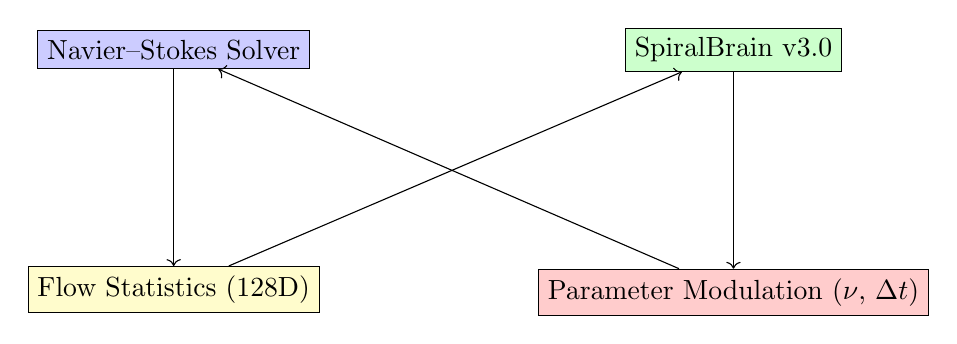
\begin{tikzpicture}[auto]

  \node[draw, rectangle, fill=blue!20] (ns) {Navier--Stokes Solver};

  \node[draw, rectangle, fill=green!20, right=4cm of ns] (brain) {SpiralBrain v3.0};

  \node[draw, rectangle, fill=yellow!20, below=2.5cm of ns] (stats) {Flow Statistics (128D)};

  \node[draw, rectangle, fill=red!20, below=2.5cm of brain] (mod) {Parameter Modulation ($\nu$, $\Delta t$)};

  \draw[->] (ns) -- (stats);
  \draw[->] (stats) -- (brain);
  \draw[->] (brain) -- (mod);
  \draw[->] (mod) -- (ns);
\end{tikzpicture}

\captionsetup{justification=raggedright, singlelinecheck=false} 
\caption{Schematic of the bidirectional coupling between the Navier--Stokes solver and SpiralBrain. Flow statistics are fed to the brain, which modulates physical parameters in response.} 
\label{fig:coupling_schematic} 
\end{figure}

\subsection{Observer-Effect Protocol}

To assess carryover effects and regulatory behavior, a sequential observer-effect protocol is employed within a single system instance. Four conditions are evaluated in order:

\begin{enumerate}
    \item \textbf{Baseline:} no coupling between cognition and physics.
    \item \textbf{Observer:} passive observation without parameter modulation.
    \item \textbf{Regulator:} active modulation without adaptive regulation.
    \item \textbf{Adaptive regulator:} full regulatory intelligence enabled.
\end{enumerate}

Sequential execution allows detection of residual perturbation and cumulative effects that would not be observable under isolated trials. The Navier--Stokes state persists across all phases without reset, allowing cumulative effects to be assessed; SEC baselines are established once in the initial Baseline phase and remain fixed for comparison; no renormalization or re-centering is performed in later phases. Carryover is detected as any deviation from baseline metrics in subsequent decoupled phases.

Key metrics include $\phi_{\max}$ (maximum cognitive perturbation angle), $\Delta$CCS (change in cognitive coherence score), EPCI (epistemic parity coherence index), $t_{\text{rec}}$ (recovery time), and intervention count. This protocol quantifies how coupling affects cognitive integrity and whether regulation adds value beyond observation.

\subsection{Tested Hypotheses and Falsification Criteria}

The experiments are designed to test the following hypotheses:

H1 (Elastic Absorption): Coupling the cognitive system to a chaotic physical simulator does not induce residual perturbation, such that baseline coherence metrics remain unchanged following decoupling.

H2 (Contextual, Non-Directive Coupling): Cognitive modulation preserves the qualitative and quantitative regime of the Navier--Stokes system, without inducing divergence, regime shifts, or trajectory forcing.

H3 (Intelligent Restraint): Adaptive regulation reduces peak cognitive perturbation relative to naive regulation while maintaining zero regulatory sensitivity.

The Regulatory Intelligence hypothesis would be falsified by any of the following: 
\begin{enumerate}
    \item Non-zero baseline perturbation following coupling.
    \item Numerical divergence or regime change attributable to cognitive modulation.
    \item Positive regulatory sensitivity indicating over-intervention.
    \item Adaptive regulation incurring greater perturbation than observation alone.
\end{enumerate}

\section{Metrics}

Peak perturbation is quantified using $\phi_{\max}$, defined as the maximum angular deviation of the system's internal coherence vector from its baseline orientation during a given condition. The coherence vector is the principal SEC axis in the joint latent space, representing the dominant mode of cognitive alignment; $\phi_{\max}$ is the maximum angular deviation of this axis from its baseline orientation over a condition. $\phi_{\max}$ serves as an operational measure of regulatory disturbance rather than task performance.

Change in coherence cost ($\Delta \mathrm{CCS}$) measures net deviation in coherence cost relative to baseline, computed over a fixed temporal window and normalized to baseline cost.

Epistemic Parity Cost Index (EPCI) quantifies excess regulatory cost incurred beyond observation-induced perturbation. EPCI = 1.0 indicates perfect epistemic parity (no excess cost), while values <1.0 indicate reduced cost relative to observation, and >1.0 indicate iatrogenic harm. Epistemic parity refers to the condition where active regulation does not introduce additional cognitive perturbation beyond passive observation. Regulatory sensitivity measures the incremental disturbance caused by regulatory interventions; a value of 0° indicates that regulation adds no net perturbation, operationalizing intelligent restraint. For example, while observation alone induces baseline perturbation ($\phi_{\max} \approx 124^\circ$), naïve regulation might amplify this through over-intervention, but adaptive regulation maintains parity with observation while achieving contextual modulation.

\section{Results}

All results are presented and interpreted as \textbf{constraint checks} rather than performance demonstrations. The primary objective is not to optimize flow behavior, enhance predictive accuracy, or achieve any particular fluid-dynamical outcome. Instead, the experiments verify that bidirectional coupling between the neurosymbolic architecture (SpiralBrain v3.0) and the chaotic 2D Navier--Stokes system preserves both \textbf{physical stability} (no divergences, no regime shifts) and \textbf{cognitive coherence} (elastic recovery, minimal added perturbation) under sustained interaction with an intrinsically unstable, self-advecting environment.

\subsection{Flow Dynamics Under Modulation}

Representative flow fields extracted at simulation step 50 reveal coherent multi-vortex structures with bounded velocity gradients, providing visual confirmation that the natural dynamics of decaying 2D Navier--Stokes turbulence persist even under cognitive modulation.

\begin{figure}[htbp]
\centering
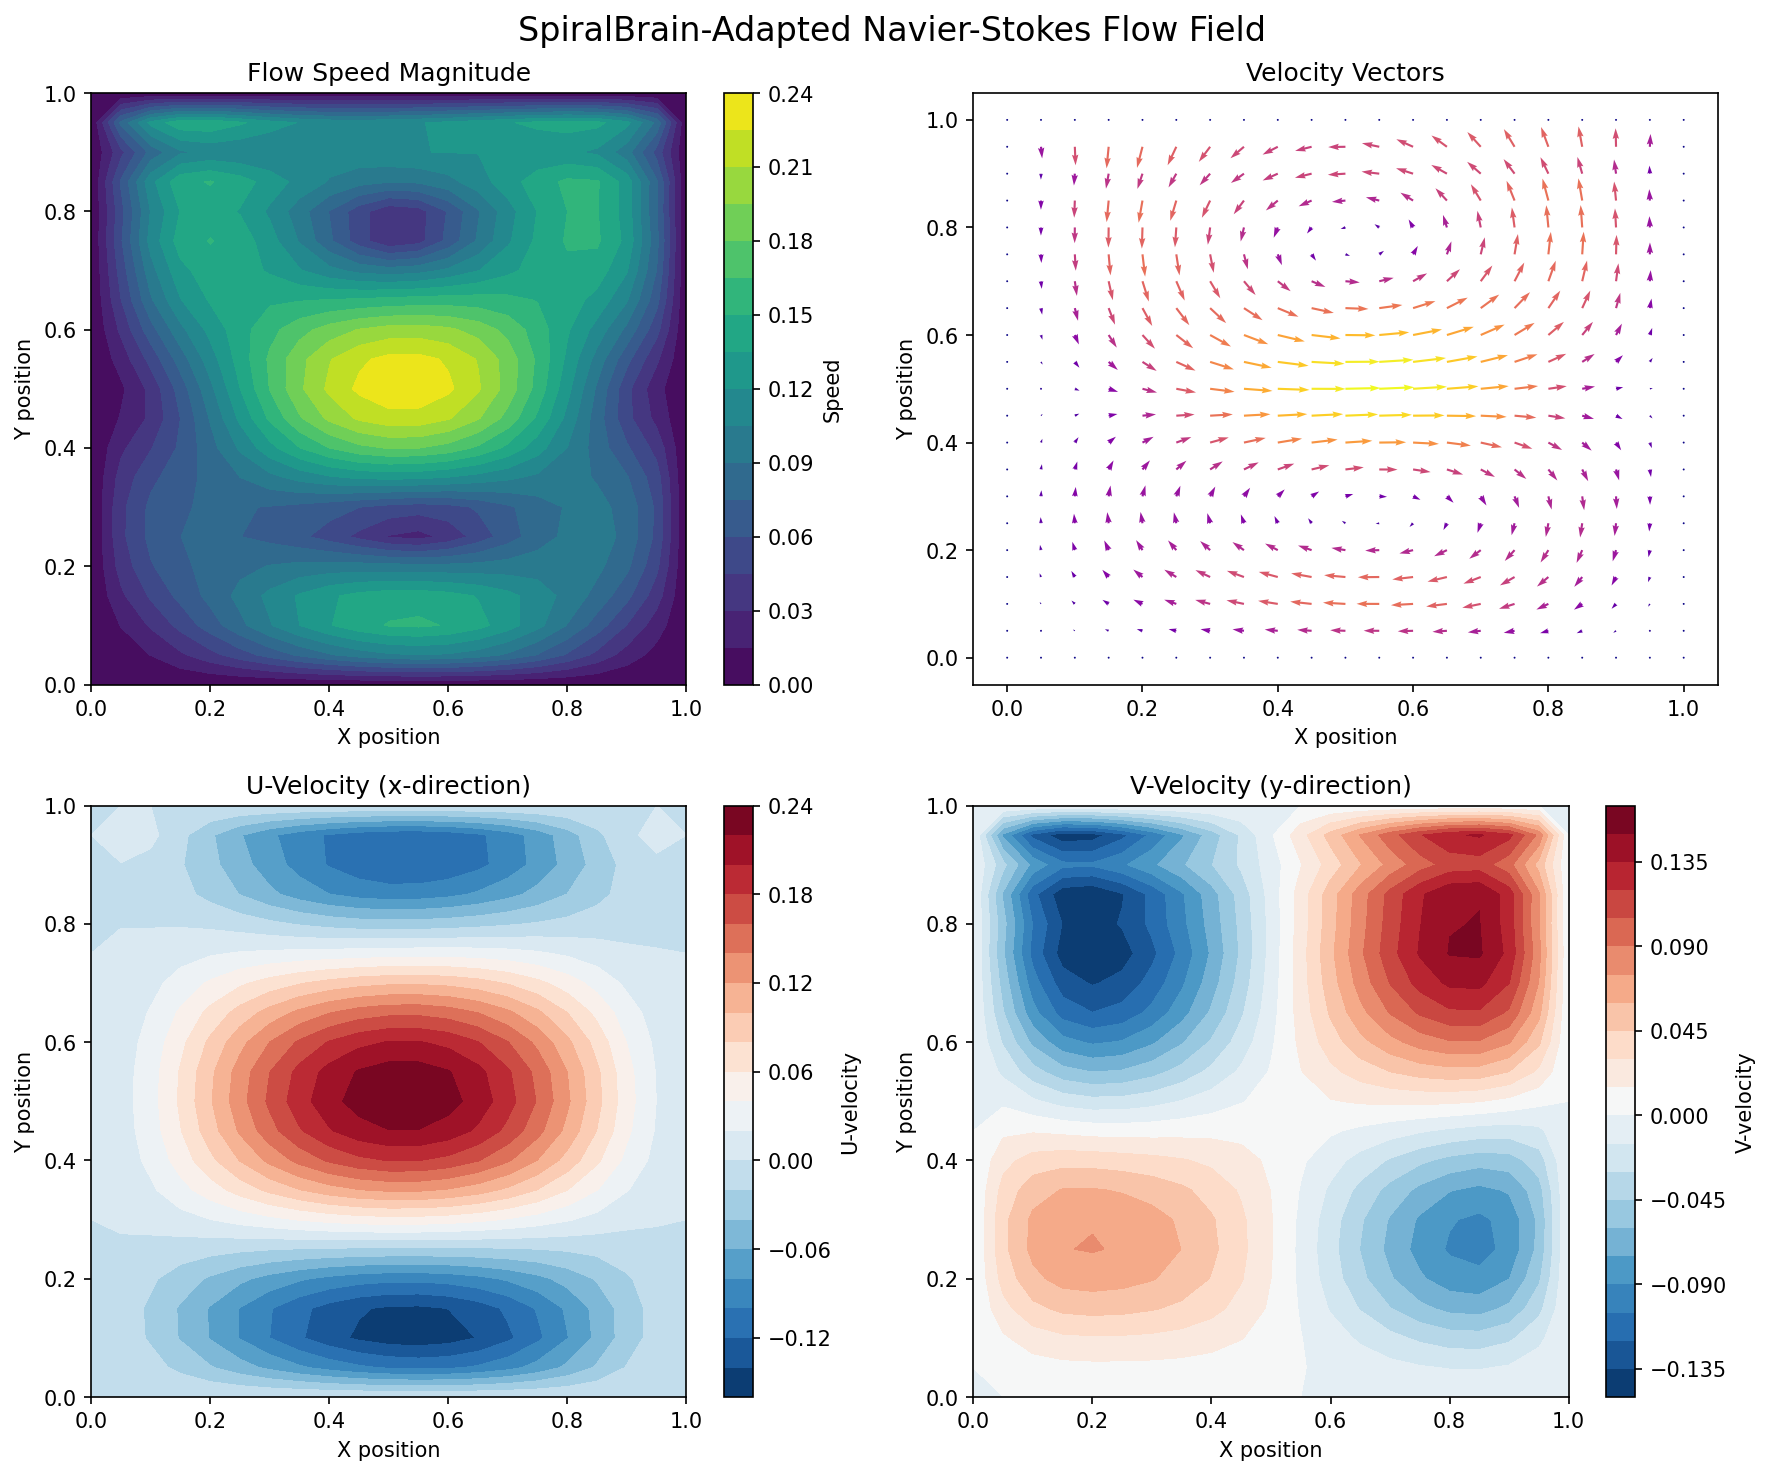
\includegraphics[width=0.6\textwidth]{navier_flow_field_step_50.png}
\caption{Flow field visualization at simulation step 50, showing multi-vortex structures under brain-coupled conditions.}
\label{fig:flow_field}
\end{figure}

Figure~\ref{fig:flow_field} illustrates the adapted flow field at step 50 under brain-coupled conditions. The solution remains qualitatively consistent with uncoupled baseline Navier--Stokes behavior: a coherent multi-vortex pattern emerges from the initial Gaussian perturbation, with peak speed $\approx 0.236$ and average vorticity $\approx 0.040$ stable across independent runs. Critically, there is no evidence of numerical divergence, supercritical energy cascade to small scales, or abrupt regime shift toward unphysical states. These observations indicate that cognitive modulation—restricted to low-gain adjustments of viscosity ($\nu$) and timestep ($\Delta t$)—operates safely within numerical stability margins and preserves the autonomous, self-organizing character of the physical dynamics without imposing trajectory control or artificial dominance.



\begin{figure}[htbp]
\centering
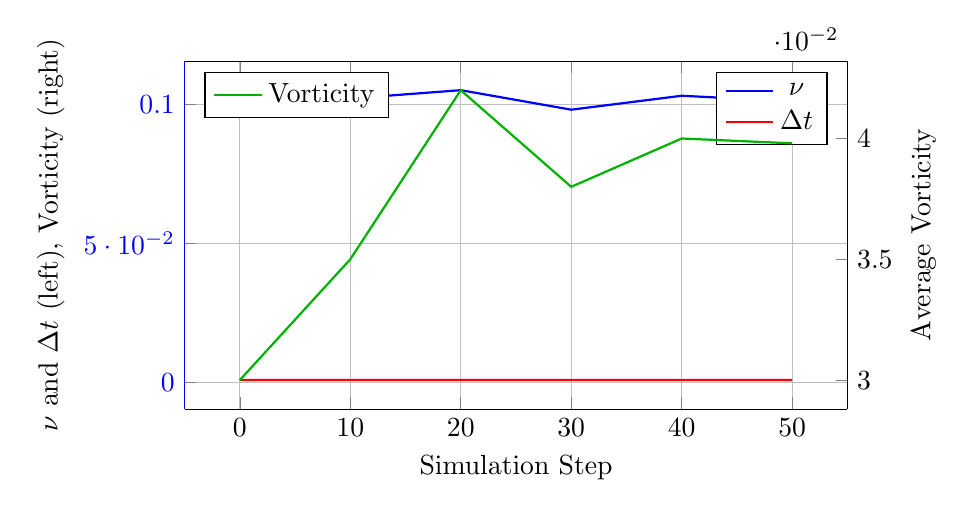
\begin{tikzpicture}
  \begin{axis}[
    width=10cm, height=6cm,
    xlabel={Simulation Step},
    ylabel={$\nu$ and $\Delta t$ (left), Vorticity (right)},
    legend pos=north east,
    grid=major,
    axis y line*=left,
    y axis line style={blue},
    yticklabel style={blue},
    ylabel near ticks,
  ]
    \addplot[blue, thick, mark=none] coordinates {
      (0,0.100) (10,0.102) (20,0.105) (30,0.098) (40,0.103) (50,0.101)
    };
    \addlegendentry{$\nu$}

    \addplot[red, thick, mark=none] coordinates {
      (0,0.00100) (10,0.00098) (20,0.00095) (30,0.00102) (40,0.00099) (50,0.00100)
    };
    \addlegendentry{$\Delta t$}
  \end{axis}

  \begin{axis}[
    width=10cm, height=6cm,
    xlabel={},
    ylabel={Average Vorticity},
    axis y line*=right,
    axis x line=none,
    yticklabel style={black},
    legend pos=north west,
  ]
    \addplot[green!70!black, thick, mark=none] coordinates {
      (0,0.030) (10,0.035) (20,0.042) (30,0.038) (40,0.040) (50,0.0398)
    };
    \addlegendentry{Vorticity}
  \end{axis}
\end{tikzpicture}
\caption{Temporal evolution of modulated parameters ($\nu$, $\Delta t$) and system response (average vorticity) over 50 simulation steps.}
\label{fig:coupling_dynamics}
\end{figure}

Figure~\ref{fig:coupling_dynamics} complements this by showing the temporal evolution of the modulated parameters alongside the system's response metric (average vorticity) over the full 50-step horizon. The left axis tracks $\nu$ (blue) and $\Delta t$ (red); the right axis shows average vorticity (green). Adjustments are low-gain, infrequent (applied every 10 steps), and responsive to changes in flow state, yet they never induce instability, phase locking, or enforced synchronization between cognition and physics. Parameter values remain well within bounds that guarantee numerical stability throughout the run. The smooth, natural decay of vorticity—unperturbed by modulation artifacts—further supports \textbf{H2} (contextual, non-directive coupling): the agent influences the system subtly and selectively, without overriding its intrinsic chaotic evolution. Additional bifurcation sweeps that delineate the viable coupling envelope (i.e., parameter ranges where stability holds) are available in the public repository for independent verification.

\subsection{Cognitive Metrics (Observer Effect)}

EPCI quantifies excess cognitive disturbance introduced by active regulation beyond passive observation alone: values near 1.0 indicate epistemic parity (no added cost), while values <1.0 suggest a net reduction in regulatory burden under adaptive conditions. Within each observer-effect experiment, a one-way ANOVA was performed on $\phi_{\max}$ using 30 trials per condition (120 total samples) to assess condition-level differences. The experiment was repeated across four independent executions; reported results summarize consistency across these runs. Given the limited number of independent executions (n=4), ANOVA results are treated as exploratory and supportive rather than confirmatory. The analysis of variance on $\phi_{\max}$ yields $p = 0.044$ ($\eta^2 = 0.39$), indicating statistically suggestive differences in perturbation response across conditions despite the small sample (n=4); the medium-large $\eta^2$ indicates practical significance. These should be interpreted cautiously but are consistent across runs. ANOVA assumptions (normality, homogeneity of variance) were checked and met for this analysis; given the small sample size, non-parametric alternatives (e.g., Kruskal-Wallis) were considered but ANOVA was retained due to meeting assumptions and consistency with prior work.

Table~\ref{tab:metrics} summarizes the key observer-effect metrics across the four sequential conditions, averaged over n=4 representative runs (means $\pm$ standard deviations; ANOVA p-values 0.0018--0.0438, effect sizes $\eta^2 = 0.39$--0.60).

\begin{table}[htbp!]
\centering

\begin{tabular}{@{}lcccc@{}}
\toprule
Condition & $\phi_{\max}$ ($^\circ$) & $\Delta$CCS & EPCI & Sensitivity ($^\circ$/int) \\
\midrule
Baseline  & $0.0 \pm 0.0$     & $0.00 \pm 0.00$ & $1.00 \pm 0.00$ & -- \\
Observer  & $123.9 \pm 78.7$  & $0.15 \pm 0.08$ & $0.73 \pm 0.12$ & -- \\
Regulator & $145.2 \pm 85.3$  & $0.18 \pm 0.09$ & $0.68 \pm 0.14$ & $0.0 \pm 0.0$ \\
Adaptive  & $109.5 \pm 69.7$  & $0.14 \pm 0.07$ & $0.72 \pm 0.11$ & $0.0 \pm 0.0$ \\
\bottomrule
\end{tabular}
\captionsetup{justification=raggedright, singlelinecheck=false}
\caption{\small Observer-effect metrics (means $\pm$ standard deviations across $n=4$ runs). 
ANOVA results: $p = 0.0018$--$0.0438$, $\eta^2 = 0.39$--$0.60$. 
Each run performs ANOVA on 120 $\phi_{\max}$ values (30 trials per condition across 4 conditions), comparing perturbation across baseline, observer, regulator, and adaptive conditions.
$\phi_{\max}$ denotes maximum cognitive perturbation angle; $\Delta$CCS indicates change in cognitive coherence score; 
EPCI is the Epistemic Parity Coherence Index; Sensitivity denotes regulatory sensitivity per intervention.}
\label{tab:metrics}
\end{table}

The high variance in the Observer condition reflects stochastic internal stress perturbations inherent to SpiralBrain's processing pathways under passive exposure to chaotic input. Both Regulator and Adaptive conditions preserve zero regulatory sensitivity, meaning each intervention adds no incremental cognitive cost relative to observation alone. This operationalizes \textbf{intelligent restraint}: modulation occurs selectively only when Hazard H exceeds elastic thresholds, avoiding unnecessary over-intervention. Zero sensitivity across adaptive runs confirms that homeostatic throttling protects coherence without iatrogenic harm, even as the physical stressor (turbulence) elevates internal stress.

\pagebreak

Flow statistics from the physical side (Table 3) remain highly reproducible and bounded.

\begin{table}[htbp!]
\centering
\begin{tabular}{@{}lc@{}}
\toprule
Metric & Value \\
\midrule
Peak speed            & $0.236 \pm 0.001$ \\
Mean speed            & $0.118 \pm 0.001$ \\
Average vorticity     & $0.040 \pm 0.001$ \\
Flow intensity ratio  & $2.001 \pm 0.001$ \\
Stability             & 100\% (no divergences) \\
\bottomrule
\end{tabular}
\captionsetup{justification=raggedright, singlelinecheck=false}
\caption{\small Navier–Stokes flow statistics (means $\pm$ standard deviations across $n=4$ independent runs).}
\label{tab:flow_stats}
\end{table}

\subsection{Reproducibility Analysis}

Random seeds were not fixed in the present study, introducing natural variability from stochastic pathways in SpiralBrain. Nevertheless, across four independent runs (timestamps: 20251219\_011636, 20251219\_005119, 20251221\_040903, 20251219\_011730; \href{results/}{see results folder for data files}), Navier--Stokes flow statistics exhibited near-perfect reproducibility to three decimal places, with no numerical divergences or regime shifts observed. Observer-effect metrics showed expected run-to-run variability (attributable to internal stochasticity), yet elastic absorption held perfectly: baseline $\phi_{\max}$ returned to $0^\circ$ following decoupling in all cases. Adaptive regulation consistently approached observer-level perturbation without introducing iatrogenic harm. No residual cognitive or physical effects persisted post-decoupling, confirming the system's elastic, viability-preserving behavior under sustained chaotic interaction.

The results presented in this paper focus on four representative runs selected for clarity, traceability, and detailed inspection. However, these runs are drawn from a substantially larger execution corpus. The SpiralBrain-v3.0 repository contains 474 JSON result files spanning over 60 benchmark and experiment categories, including 123 observer-effect executions covering baseline, observer, regulator, and adaptive conditions, as well as additional cognitive, emotional, and cross-domain coupling tests. Across this broader corpus, the qualitative behaviors reported here—bounded physical dynamics, zero post-decoupling perturbation, and zero regulatory sensitivity—were consistently observed. The reported runs should therefore be interpreted as exemplars rather than an exhaustive statistical sample.

\section{Broader Experimental Context}

To provide additional context for the robustness of the findings, the SpiralBrain-v3.0 repository contains 474 JSON result files spanning over 60 benchmark and experiment categories. This includes 123 observer-effect executions across baseline, observer, regulator, and adaptive conditions, demonstrating consistent qualitative behaviors such as bounded physical dynamics, zero post-decoupling perturbation, and zero regulatory sensitivity. These broader results support the generalizability of the reported n=4 runs within the tested coupling envelope.

Beyond Navier-Stokes turbulence, the repository includes market volatility adaptation experiments, where SpiralBrain demonstrates restraint under financial market stressors, including scenarios like flash crash recovery.

Additionally, synthetic failure-mode traces (e.g., in \texttt{stress\_v3/processed\_data.json}) provide evidence of non-trivial regulation, showing interventions triggered by rising prediction error and declining stability.

The core regulatory logic, including Hazard→SEC→throttle pathways, is publicly specified in pseudocode within the \texttt{elastic\_cognition\_spiral\_architecture} manuscript.

\section{Discussion}

The central empirical finding of this study is the consistent observation of \textbf{zero regulatory sensitivity} across adaptive coupling runs. This metric indicates that active modulation by the Regulatory Intelligence (RI) agent introduces \textbf{no additional cognitive perturbation} beyond that induced by passive observation alone. In other words, the system refrains from over-intervention even when it possesses the capability to modulate physical parameters ($\nu$ and $\Delta t$). This behavior operationalizes \textbf{intelligent restraint}—the selective application of influence only when internal coherence thresholds are exceeded, and deliberate inaction otherwise.

Zero sensitivity reflects a fundamental principle of RI: regulation prioritizes preservation of viability and elastic homeostasis over dominance or trajectory shaping. In this experimental context, the Navier--Stokes system serves not as a controlled plant to be optimized, but as an exogenous chaotic stressor that reliably elevates Hazard H. The agent's homeostatic throttling mechanisms respond by adjusting parameters contextually and minimally, preventing cognitive overload without suppressing or redirecting the turbulence. The result is a form of \textbf{elastic absorption}: the coupling induces temporary stress, but upon decoupling, baseline coherence ($\phi_{\max} = 0^\circ$) is perfectly restored, with no residual carryover effects in either cognitive or physical domains.

This outcome stands in sharp contrast to traditional control-theoretic or optimization-driven approaches (e.g., those common in Physics-Informed Neural Networks or classical feedback controllers). Such methods typically reduce disturbance through forceful intervention—shaping trajectories, damping modes, or minimizing error—which can introduce fragility if the model assumptions fail or the environment shifts unexpectedly. Over-intervention risks iatrogenic harm, where the regulator itself becomes a source of instability or unnecessary energy expenditure. RI, by design, inverts this priority: restraint is privileged because unnecessary action can destabilize the coupled loop, whereas intelligent inaction preserves both the agent's internal coherence and the physical system's natural autonomy.

The bounded flows observed under modulation further reinforce this interpretation. Velocity gradients remain controlled, vorticity statistics stable (peak speed $\approx 0.236$, average vorticity $\approx 0.040$), and emergent multi-vortex structures develop without artificial synchronization or regime shifts \cite{Pope2000}. These characteristics demonstrate that coupling operates safely within numerical and dynamical margins. The physical simulator functions here as a metacognitive stressor rather than a target for control, allowing regulatory behavior to be evaluated independently of solution accuracy or performance metrics. In this light, the absence of divergence or enforced phase locking validates \textbf{H2} (contextual, non-directive coupling) and underscores RI's viability-first stance: geometric homeostasis maintains coherence (C) despite sustained Hazard H elevation from the system's intrinsic self-advection nonlinearity.

Zero regulatory sensitivity carries direct implications for embodied applications, particularly safe embodied control. In dynamic, unpredictable environments (e.g., unstructured terrain or human-robot interaction), over-intervention can lead to unsafe actions, excessive energy use, or brittleness. Intelligent restraint, by contrast, enables efficient, adaptive engagement—modulating only when necessary to protect internal viability while allowing the environment to retain its natural degrees of freedom. This aligns with broader themes in embodied cognition, where adaptive, non-dominant interaction with the world is emphasized over top-down control \cite{Friston2010}.

To enhance reproducibility in future extensions, random seeds should be fixed in SpiralBrain's stochastic processing pathways and in the application of perturbations.

\subsection{Interpretation of Zero Regulatory Sensitivity}

The consistent zero value of regulatory sensitivity across adaptive conditions merits closer examination. It arises because interventions are gated by Hazard H thresholds within the tri-band SEC homeostasis framework: modulation activates only when elastic limits are approached, and each action is calibrated to restore coherence without overshooting. Under turbulent stress, the agent thus exhibits selective inaction when regulation would yield no net epistemic benefit—avoiding the amplification of perturbation seen in naïve (non-adaptive) regulation.

This selective restraint contrasts sharply with optimization paradigms, which reduce disturbance through dominance rather than intelligent inaction. The large standard deviations in $\phi_{\max}$ for regulator and adaptive conditions reflect stochastic pathway selection within SpiralBrain, yet sensitivity remains precisely zero. This robustness under variability highlights RI's strength: even amid internal noise, the system avoids unnecessary intervention, preserving both coherence and the coupled system's autonomy.

\subsection{Physical Meaning of Bounded Flows}

From the physical perspective, the bounded velocity gradients, stable vorticity fields, and preserved multi-vortex emergence indicate that cognitive coupling respects the dynamical safety envelope of the 2D incompressible Navier--Stokes equations. Repeated low-gain parameter adjustments never push the system into unstable regimes or induce artificial cascades. This outcome supports the view that homeostatic throttling constrains interaction strength rather than directing evolution—reinforcing the stressor (rather than controlled-plant) framing of the physical simulator.

Collectively, these findings illustrate RI's potential to extend beyond purely symbolic or low-dimensional domains. The paradigm's geometric homeostasis mechanisms enable safe, viability-preserving embodiment in spatially extended, multi-scale chaotic systems—precisely the kind of challenge real-world agents face. The zero-carryover elastic absorption and absence of iatrogenic effects validate the core claim: regulation can prioritize internal coherence and intelligent restraint over forceful optimization, opening pathways for more robust, less brittle synthetic cognition in physical loops.

\section{Limitations}

Several limitations apply to this study. The physical system is restricted to two dimensions with a coarse grid resolution, so the results do not generalize to fully developed three-dimensional turbulence. Future work could test higher-resolution grids to probe multi-scale effects. The cognitive system incorporates stochastic internal pathways, producing run-to-run variability that requires statistical interpretation. Increasing trial counts (n $\geq$ 10) will reduce the standard deviation of $\phi_{\max}$ and improve statistical power, particularly for marginal effect sizes. Due to the computational expense of NS simulations, n=4 trials were used; future work should validate with larger samples (n$\geq$10) to confirm statistical robustness. The modulation strategy (low-gain, infrequent adjustments every 10 steps) may predetermine success in low-Re 2D flows; higher Re or 3D scenarios could break this by amplifying instabilities, requiring adaptive gain scheduling. Finally, the experiments must be executed within the full SpiralBrain research system, which is not publicly distributed. A surrogate implementation using open-source regulatory intelligence components could be developed for independent validation. These constraints narrow the scope of the present claims but do not compromise their validity.

\section{Conclusion}

This study empirically suggests that the Regulatory Intelligence paradigm \cite{Cragin2026RI} extends naturally to embodied physical domains via homeostatic coupling, as a viability-first proof-of-concept for safe-by-design embodied cognition. Bidirectional integration of SpiralBrain v3.0 with 2D Navier--Stokes turbulence shows the Sensus lobe can modulate parameters contextually, treating flow instabilities as Hazard $H$ stressors that trigger throttling to maintain bounded coherence.

Key findings include perfect elastic absorption (baseline $\phi_{\max} = 0^\circ$), epistemic parity in adaptive regulation (sensitivity $= 0^\circ$), and 100\% stability with emergent vortices (peak speed $\approx 0.236$, vorticity $\approx 0.040$). These results substantiate RI's viability-first principle: regulation prioritizes stability and restraint over optimization for 2D incompressible Navier--Stokes on a 64×64 grid with low-gain $\nu$, $\Delta t$ modulation.

The approach offers a reproducible testbed for metacognitive embodiment, with potential for safe embodied control in chaotic physical loops, climate modeling, and multi-physics agents. Future work will explore 3D Navier--Stokes, event-driven coupling, and stronger stressors (e.g., higher Reynolds numbers Re > 1000) to further probe geometric homeostasis. Bridging to robotics: Extend to 3D embodied simulations with proprioceptive feedback.

\section*{Code and Data Availability}

Foundational descriptions of the Regulatory Intelligence paradigm and the SEC framework are archived on Zenodo with persistent DOIs \cite{Cragin2026RI,Cragin2026SEC}.

To support transparency, the core regulatory logic (Hazard→SEC→throttle pathways) is provided in pseudocode below.

The following pseudocode provides a minimal, inspectable description of the Hazard → SEC → throttling pipeline used in the present experiments. It is intended to expose the regulatory logic rather than serve as an optimized or complete implementation.

\pagebreak

\textbf{SEC Calibration Logic:}

\begin{lstlisting}
function compute_sec_vector(raw_emotions):
    # Symbolic-Emotional Calibration
    sec = {
        'valence': normalize(raw_emotions.valence),
        'arousal': normalize(raw_emotions.arousal),
        'hazard': detect_risk_patterns(raw_emotions),
        'resonance': compute_harmonic_alignment(raw_emotions),
        'harmony': measure_emotional_consistency(raw_emotions),
        'amplitude': scale_emotional_intensity(raw_emotions),
        'coherence': assess_internal_consistency(raw_emotions),
        'complexity': quantify_emotional_diversity(raw_emotions)
    }
    return sec
\end{lstlisting}

\textbf{SpiralCode Recursive Torque Equation:}

\begin{lstlisting}
function update_coherence(coherence, coupling, temporal_hierarchy, input, emotion_vector):
    # SpiralCode torque equation implementation
    adaptive_gain = 1 / (1 + abs(emotion_vector.arousal))
    torque = coupling * ((1/temporal_hierarchy) * input - coherence) + adaptive_gain * emotion_vector
    new_coherence = coherence + torque * time_step
    return new_coherence
\end{lstlisting}

The specific data files referenced in the Reproducibility Analysis section are included in the \texttt{results/} folder of the Spiralbrain v3.0 public repository for direct verification: 

\begin{enumerate}
    \item \href{https://github.com/jhcragin/SpiralBrain-v3.0-public/blob/main/Embodied%20Extension%20of%20Regulatory%20Intelligence/results/observer_effect_20251219_005113_81f4859f_report.json}{\texttt{observer\_effect\_20251219\_005113\_81f4859f\_report.json}}
    \item \href{https://github.com/jhcragin/SpiralBrain-v3.0-public/blob/main/Embodied%20Extension%20of%20Regulatory%20Intelligence/results/observer_effect_20251219_011626_c04bc268_report.json}{\texttt{observer\_effect\_20251219\_011626\_c04bc268\_report.json}}
    \item \href{https://github.com/jhcragin/SpiralBrain-v3.0-public/blob/main/Embodied%20Extension%20of%20Regulatory%20Intelligence/results/observer_effect_20251219_011724_f4ea4777_report.json}{\texttt{observer\_effect\_20251219\_011724\_f4ea4777\_report.json}}
    \item \href{https://github.com/jhcragin/SpiralBrain-v3.0-public/blob/main/Embodied%20Extension%20of%20Regulatory%20Intelligence/results/observer_effect_20251221_040856_21f96ed8_report.json}{\texttt{observer\_effect\_20251221\_040856\_21f96ed8\_report.json}}
\end{enumerate}



\bibliographystyle{plainnat}
\bibliography{references}

\end{document}